\documentclass[a4paper,12pt]{article}
\usepackage{blindtext}
\usepackage[utf8]{inputenc}
\usepackage[russian]{babel}
\usepackage{graphicx}
\usepackage[left=2cm,right=2cm,top=2cm,bottom=2cm,bindingoffset=0cm]{geometry}
\usepackage{verbatim}
\usepackage{textcomp}
\usepackage{xcolor}
\usepackage{hyperref}
\definecolor{urlcolor}{HTML}{799B03}
\definecolor{linkcolor}{HTML}{799B03}
\hypersetup{pdfstartview=FitH,  linkcolor=linkcolor, urlcolor=urlcolor, colorlinks=true}
\graphicspath{ {./images/} }
\title{Nbgrader.}
\author{Винецкая Полина}
\begin{document}
\maketitle
\tableofcontents
\section{Установка.\small \textit{ Для работы с сервером не нужно}} 

Для установки nbgrader откройте терминал и введите команду:
\begin{verbatim}
pip install nbgrader
\end{verbatim}
или
\begin{verbatim}
conda install jupyter
conda install -c conda-forge nbgrader,
\end{verbatim}
если вы используете анаконду.

Для получения доступа к возможностям учителя, 
необходимо установить расширения:
\begin{verbatim}
jupyter nbextension install --sys-prefix --py nbgrader --overwrite
jupyter nbextension enable --sys-prefix --py nbgrader
jupyter serverextension enable --sys-prefix --py nbgrader
\end{verbatim}
Первое расширение необходимо для создания заданий.
Для assignment list, formgrader, и validate необходимы оба расширения.
\section{Создание курса} Есть два пути: создать свой курс с нуля или использовать шаблон.
\subsection{Шаблон}

Команда
\begin{verbatim}
nbgrader quickstart course_id 
\end{verbatim}
создаст курс с названием course\underline{ }id и наполнением из 2 заданий и 2 студентов. На примере шаблона проще всего разобраться в работе nbgarder'a
\subsection{Создание своего курса}

Создается папка со структурой, описанной в п.3, файлом nbgrader\underline{ }config.py и базой данных. Мне кажется, удобнее  редактировать шаблон, т.к. повторить вручную всю структуру курса довольно сложно.
\section{Структура}
\subsection{Команды}

Команды nbgrader строятся следующим образом:
\begin{verbatim}
{course_directory}/{nbgrader_step}/{student_id}/{assignment_id}/{notebook_id}.ipynb
\end{verbatim}
course\underline{ }directory -- корневая папка, в которой хранится все (информация о классе, заданиях и т.д.)

nbgrader\underline{ }step -- команда (проверить, забрать, раздать задания и т.д.). Есть тонкости с тем, где запускать команды и где будет видно их результат. Далее подробнее.

*\underline{ }id можно заменить звездочкой, если нужно выполнить команду для всех элементов.
\subsection{Вид}
\subsubsection{Учитель}
Структура nbgrader'a устроена так: есть две папки: корневая (couse\underline{ }directory) и обменная (exchange). Корневая папка содержит в себе информацию о курсе, учениках, заданиях. В ней хранятся решения преподавателя, и к ней доступа у учеников нет.

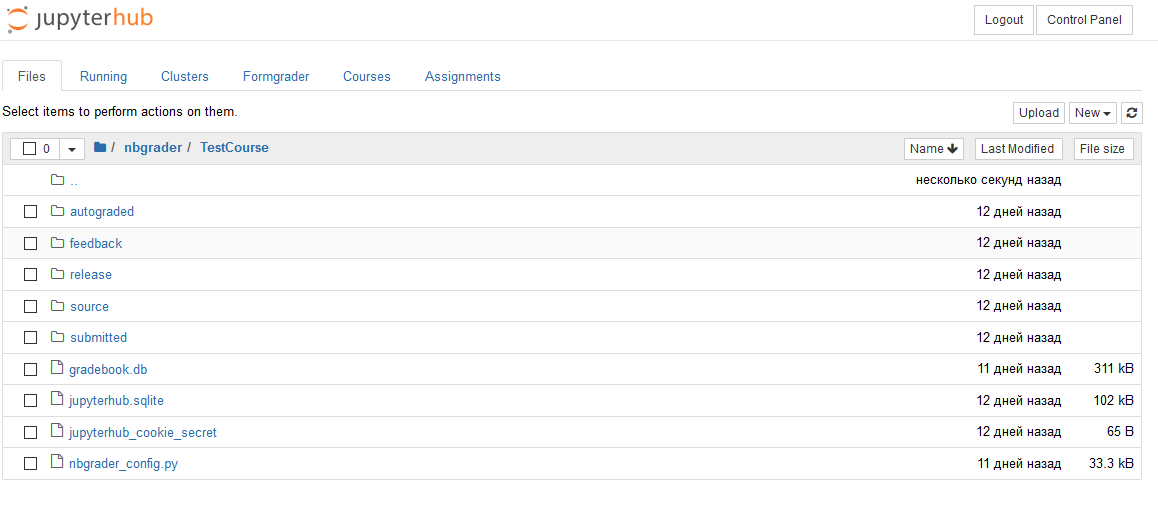
\includegraphics[width=\textwidth]{grader_root_directory}

Обменная папка создана для обмена между учениками и преподавателем, в ней хранятся: а) Выложенные задания учителя без решений б)Решения студентов в)Фидбэки учителя и nbgrader на каждое задание каждого ученика. При работе с сервером напрямую в нее доступа ни у кого нет.

\paragraph{Для работы без сервера}
Для работы со сторонним облаком вроде Dropbox студенты и учитель должны поставить nbgrader локально. "Студенческая" версия ставится в две строчки и требует только анаконду и питон версии не ниже 3(раздел 7). Можно установить на почти любую операционную систему, но как показала практика, не на 32-битную.

 Основная проблема, с которой столкнется преподаватель, если у учеников не стоит nbgrader, это безумные таймстемпы, без которых nbgrader не будет проверять задания и отсылать фидбэки. Пока я не нашла способа отключить их, поэтому, если ученики не ставят себе nbgrader, преподавателю придется таймстемпы генерировать с помощью какого-то скрипта. 

\paragraph{Что есть в папке курса}

gradebook.db --  База данных типа sQlite database, находится в \begin{verbatim} {course_directory}/gradebook.db.\end{verbatim}
Внутрь нее лезть обычно необходимости нет, nbgrader все манипуляции выполняет сам. 

nbgrader\underline{ }config.py -- также находится в корневой папке курса. Хранит всю информацию о курсе, связанную с базой данных(адрес обменной папки, информация об учениках и т.д)

Например, 
\begin{verbatim}
c.CourseDirectory.course_id = "course101" -- метод, задающий id курса
\end{verbatim}

\subsubsection{Студент}
У студента тоже есть корневая папка, соответствующая курсу (можно подписаться на нескольно разных курсов,тогда и корневых папок будет несколько). Однако в ней отображаются только те задания, на которые студент подписался (функция fetch). 
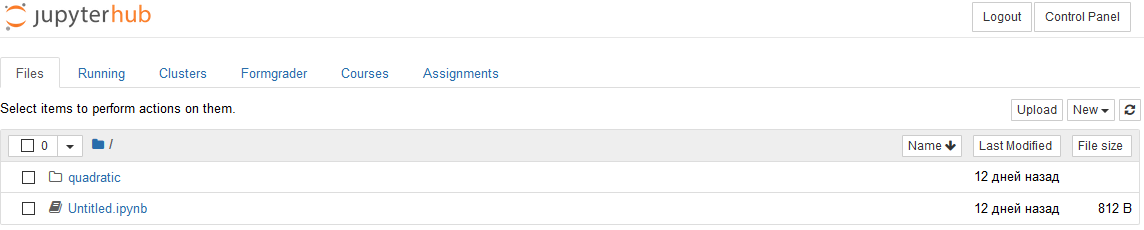
\includegraphics[width=\textwidth]{student_root_directory}

\section{Работа с nbgrader}

Все, необходимое учителю, укладывается в схеме
\begin{verbatim}
Make assignment -- Generate -- Release -- Collect -- Grade -- Feedback
\end{verbatim}
\subsection{Formgrader}

Расширение, позволяющее работать не через командную строку, а прямо в Jupyter. 

Если все расширения из пункта 1 были установлены верно(если вы устанавливаете nbgrader локально), в Jupyter появится вкладка:
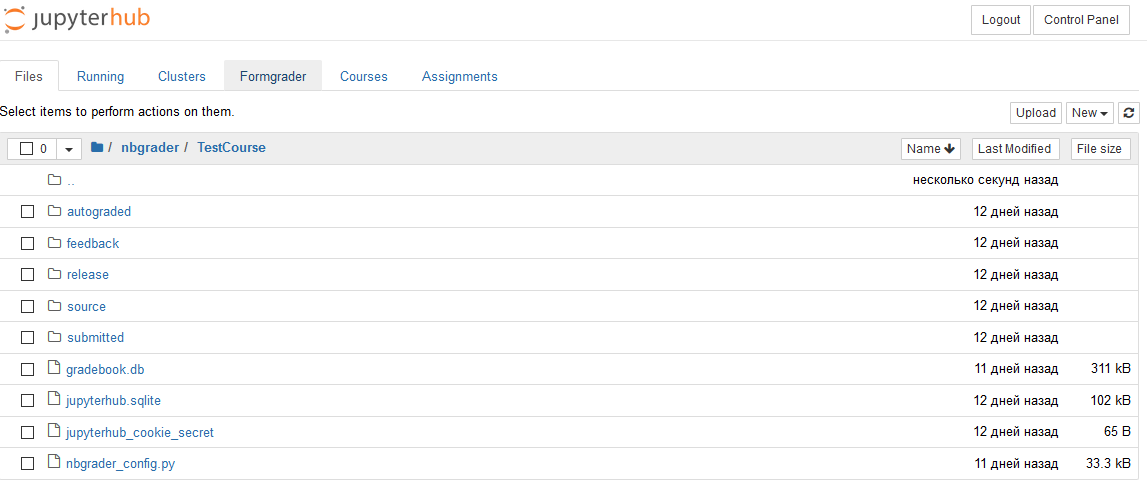
\includegraphics[width=\textwidth]{formgrader_tab1}
\paragraph{Возможная проблема (не для сервера)}
Если вы видите табличку \grqq The course id has not been set in nbgrader\underline{ }config.py\grqq, а в графе formgrader \grqq No data available in table\grqq , значит, вы запустили Jupyter находясь не в корневой папке курса.
\subsection{Создание задания}
\subsubsection{С помощью Formgrader}

Здесь все просто: нажимаете +add assigment, добавляете имя и время дедлайна(опционально).

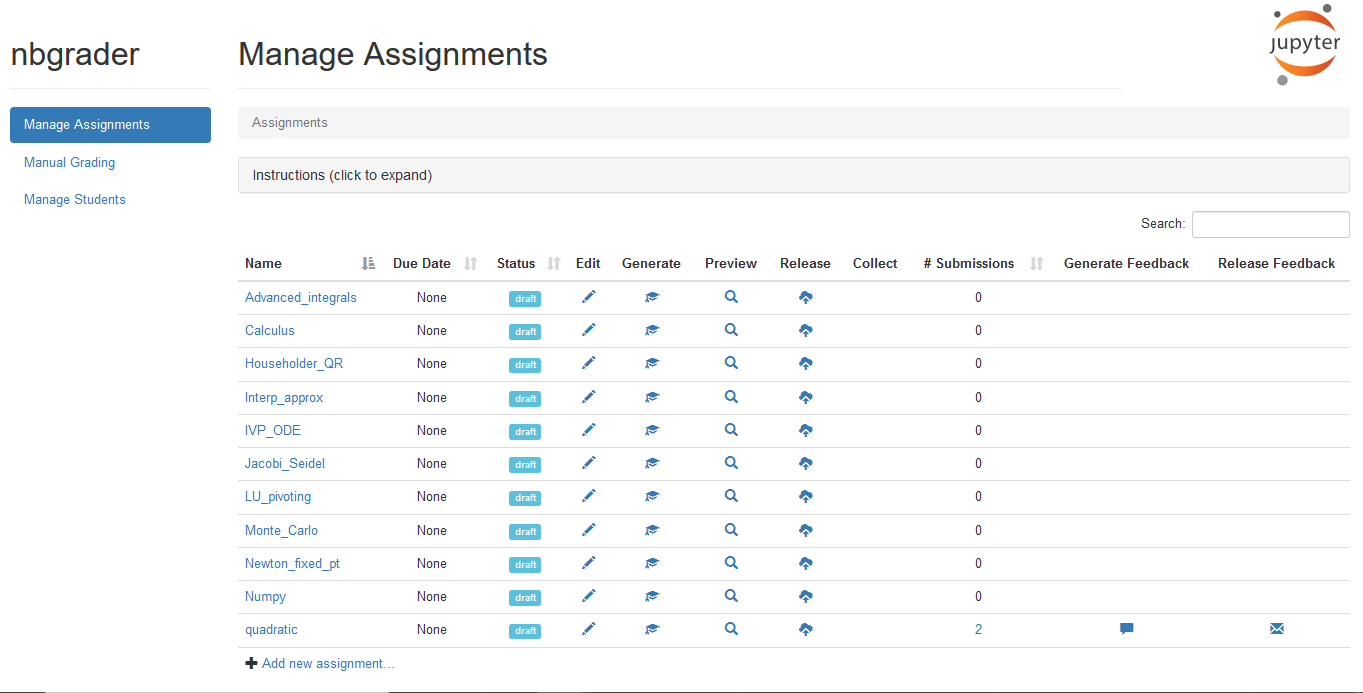
\includegraphics[width=\textwidth]{formgrader_tab2}
В таблице formgrader появится имя задания, в эту папку нужно поместить ноутбуки с задачами (их может быть несколько)
(Зайти в папку можно кликнув на имя в таблице)
\subsubsection{Командная строка}

Все задания, созданные вами, но еще не опубликованные, хранятся в папке курса в разделе source, поэтому для добавления задания с названием assigment\_id можно просто создать папку course\_id/source/assigment\_id и в нее помеситить задачи, однако тогда надо обновить соответствующую строку в nbgrader\_config.py.
\subsection{Добавление тестов}

Для того, чтобы сделать задачи удобоваримыми для nbgrader, нужно добавить тесты и ответы к ним.
\paragraph{Важно}Nbgrader прячет от студентов решения и тесты, если использовать соответствующие бракеты. Все бракеты и их содержимое будут скрыты от студента и заменены на фразы типа  \grqqВведите решение\grqq.
В ноутбуке с заданием нужно нажать View -- Cell Toolbar: откроются все возможности nbgrader.

Нажмите Create Assigment. В правом углу каждой ячейки появится окошко с выбором вида этой ячейки, а после выбора появится id этой ячейки (по этим id nbgrader будет ориентироваться при проверке и прятать нужные ячейки от студентов при релизе). Слева от id появится ячейка с количеством баллов за задание. Ячейки, подсвечивающиеся синим, не будут доступны студентам в своем первоначальном виде.

\subsubsection{Read only}

Обычный комментарий. Отличается от ячейки markdown тем, что является неизменяемым для студента. В formgrader это отмечено знаком замка в левом углу ячейки.
\paragraph{Важно}
В зависимости от версии nbgrader, функционал таких ячеек изменяется. На текущей версии все работает так:

При генерации задания содержимое ячейки записывается в базу данных. Во время проверки nbgrader заменяет содержимое этой ячейки в файле студента на то, что было сохранено в базе данных на момент релиза. То есть например, вариант удалить ячейку с тестами и получить 100\% не прокатит, nbgrader восстановит ячейку и проверит код. Именно поэтому тесты и решения пишутся в разных ячейках: тесты также обладают функциями ячейки Read-only. 
\subsubsection{Manually graded task}

Задания, требующие индивидуальнной проверки учителем каждого ученика и нескольких ячеек, например \grqqприведите графики, придумайте тесты, хорошо показывающие недостатки модели\grqq. В самой ячейке вводится только текст задания, ученик (наверное?) создаст новые ячейки, в которых выполнит задание.
Для этого типа ячеек можно добавить решение в бракетах === BEGIN MARK SCHEME === ... === END MARK SCHEME ===,
например, для облегчения работы ассистентам. Эта часть будет скрыта от студента.

\subsubsection{Manually graded answer}

Задания, требующие индивидуальнной проверки учителем каждого ученика, например \grqqобъясните эффект\grqq или \grqqнапишите формулу\grqq. Выполняются в той же ячейке.
\paragraph{Важно}Сам текст задания нужно писать в другой ячейке, вида Read only, так как содержимое Manually graded answer ячеек nbgrader заменит на фразу YOUR ANSWER HERE в версии студента.

\subsubsection{Autograded answer}

Доступны только для ячеек с кодом. В бракетах \#\#\# BEGIN SOLUTION ... \#\#\# END SOLUTION нужно написать решение. 
Если написать решение, но не использовать бракеты, nbgrader скроет от студента все содержимое ячейки, но исключения не выдаст. Баллы за эту ячейку не выставляются, так как критерием являются тесты. 

\subsubsection{Autograder tests}

Доступны только для ячеек с кодом. Необходимо ипользовать функции типа numpy.allclose или похожие. Если все тесты проходят, студент получает число баллов в ячейке. Хотя бы 1 тест падает -- 0 баллов за задание.
Если вы хотите чтобы тесты были скрыты от студента, можно использовать бракеты \#\#\# BEGIN HIDDEN TESTS и \#\#\# END HIDDEN TESTS.

\paragraph{Важно}
Эта функция Особенно важна для тестирующих ячеек, которые всегда помечены как read-only. Из-за того что механизм автопровеки выставляет студенту максимальный балл в случае прохождения всех тестов, простым способом обойти это было бы просто удалить или закомментировать тесты. Поэтому ячейки read-only игнорируют все изменения, сделанные студентом. А если работать через сервер, эти ячейки будут просто не кликабельны.

\paragraph{Очень важно}
Если изменить количество ячеек при работе (на сервере так сделать невозможно), залить задания получится, а проверить нет. Nbgrader каждой ячейке дает индивидуальный id, и если хотч бы одну из ожидаемых ячеек не находит, работать отказывается.
\subsection{Проверка}
\subsubsection{Formgrader}

Чтобы проверить адекватность тестов, достаточно нажать кнопку Validatе на панели Jupyter сверху. Nbgrader запустит ячейки, и в случае, если ваше решение успешно обработает все тесты, выдаст:
\grqq Success! Your notebook passes all the tests.\grqq
\\В противном случае вы увидите на экране \grqqобвалившиеся\grqq ячейки.
\subsubsection{Командная строка}

Для командной строки существует команда nbgrader validate assignment\underline{ }id. Однако чтобы проверить нужный ноутбук, нужно указать его адрес относительно корневой папки курса.
\begin{verbatim}
nbgrader validate source/assigment_id/problem_id.ipynb
\end{verbatim}
\subsection{Generate}

Создает версию для релиза (ту, которую увидит студент), убирая ответы и скрытые тесты из задания, лежащего в папке source. Однако студенту сгенерированные задания все еще будут недоступны.

\subsubsection{Formgrader}

Чтобы сгенерировать задание, надо перейти во вкладку formgrader и нажать на значок шапки в графе generate напротив соответствующего задания. Вы увидите окно log output.
\paragraph{Возможная проблема}
В папке source должен лежать файл header.ipynb; если его там нет, его нужно скачать и вставить. По смыслу это шапка, в которой студент напишет информацию о себе, без нее будет выдаваться странная ошибка.
Для того чтобы увидеть версию для релиза, можно нажать на значок лупы в строчке с соответствующим заданием во вкдадке formgrader.
\subsubsection{Командная строка}

Для командной строки существует функция nbgrader generate assignment\underline{ }id.
Перед использованием команды убедитесь, что нужный ноутбук лежит по адресу 
\begin{verbatim}
{course_directory}/source/{assignment_id}/{notebook_id}.ipynb
\end{verbatim}
Сгенерированное задание будет лежать по адресу
\begin{verbatim}
{course_directory}/release/{assignment_id}/{notebook_id}.ipynb
\end{verbatim}
В результате папки source и release будут аналогичны по структуре, только в первой будут лежать ноутбуки преподавателя, с решениями и тестами, а во второй -- те же файлы, но зацензурированные, для учеников.

Если вы хотите проверить через командную строку, что ваши действительно спрятаны в версии для студента, можно использовать команду
\begin{verbatim}
nbgrader validate --invert release/{assignment_id}/{notebook_id}.ipynb
\end{verbatim}
Если все хорошо, то есть файл на месте, и все тесты обвалились, вывод будет следующим:
\grqq Success! The notebook does not pass any tests\grqq
\subsection{Публикация}

При работе локально релиз происходит так: по адресу(про него в 4.5.0) nbgrader создает папку с названием курса(папку для обмена), а в ней две директории: outbond для релиза и inbond для сбора(о ней в разделе 4.6). \\То есть результат действия \grqqпубликация задания\grqq -- это перемещение ноутбуков, соответствующих этому заданию в папку outbond из папки course\underline{ }directory/release.
Папка outbond по организации и содержанию выглядит точно так же, как и release в папке курса, однако находится не в папке курса. (По факту папка курса должна быть доступна только учителю, а outbond расшарена ученикам).

Для работы с сервером таких проблем нет.
\subsubsection{Папка exchange}
В файле get\underline{ }config.py можно вписать адрес папки для обмена между студентами и преподавателем:
\begin{verbatim}
c = get_config()

c.CourseDirectory.course_id = "example_course"
c.Exchange.root = "/tmp/exchange" например
\end{verbatim}
В последней строке вписываем путь к папке обмена, которая уже должна существовать и все пользователи дожны иметь право изменять/удалять/создавать файлы.
Кнопка release во вкладке formgrader перемещает ноутбуки по этому адресу. Если ничего не указывать, адрес папки обмена:
\begin{verbatim} /srv/nbgrader/exchange/course_id/outbound/ \end{verbatim}
\subsubsection{Formgrader}

Тут снова все просто: в вкладке formgrader нужно нажать на значок в виде облака для релиза, и на крестик для того, чтобы релиз отменить. 
\paragraph{Возможная проблема}
Если вы поменяли адрес папки обмена, но релиз произошел по старому адресу, перезапустите ядро Jupyter.
\subsubsection{Командная строка}

Команда nbgrader release assignment\underline{ }id выполняет релиз по адресу, указанному в файле get\underline{ }config.py.
\subsection{Сбор}

\paragraph{(если у студента не установлен nbgrader, а сервер не используется)}
Такого не предполагает функционал, поэтому часть автоматических действий перекладывается на учителя.

В папке
 \{exchange\underline{ }directory\}/\{course\underline{ }id\}/inbond/ должны лежать папки студентов со структурой
/\{student\underline{ }id+assignment\underline{ }id+timestamp\}/.ipynb
\\Пример: 
\begin{verbatim}
/tmp/exchange/TestCourse/inbound/vivanov+quadratic+2020-04-18 17:50:45.884871 UTC/
/quadratic_exercise.ipynb
\end{verbatim}
\paragraph{Проблема}Я пока не нашла способа избежать такой сложной структуры, так как она создается nbgrader'ом, когда студенты отсылают свои решения. Возможно он есть. Если изменить имя папки, функция collect работать не будет.
\subsubsection{Formgrader}

во вкладке formgrader в столбике \#submissions будет указано количество решений. Для того, чтобы их \grqqзабрать\grqq, надо нажать на облачко в графе collect.
\subsubsection{Командная строка}

Функция nbgrader collect 
\subsection{Проверка}

\subsubsection{Автопроверка}

Для автопроверки нужно нажать на количество сданных решений,а затем на значок молнии. nbgrader выставит баллы за каждое автоматически проверенное задание и изменит статус ассигмента. 
\subsubsection{Вручную}

Если есть задания, требующие проверки вручную, вам об этом напомнит статус задания. Чтобы выполнить проверку, нужно выбрать вкладку Manual Grading слева в форме formgrader. Далее нажать на задание, затем на ноутбук,и щелкнуть на первую работу из сданных. Откоется окно, в котором около кажно из ячеек можно выбрать количество баллов, в том числе изменить оценку, выставленную nbgrader автоматически. Сверху есть две вкладки ← Prev и Next → , с помощью которых можно переключаться между ноутбуками учеников.
\subsection{Feedback}

С формированием фидбэка все просто: после проверки задания во вкладке formgrader нужно нажать на значок письма во вкладке Generate Feedback. В корневой папке, по адресу /feedback/\{student\_id\}/\{assignment\_id\}/ будет лежать фидбэк в формате .html
А вот с отправкой фидбэка есть проблемы. Из-за отсутствия таймстэмпов(см) nbgrader отказывается перемещать файлы в обменную папку. Пока что есть два варианта решения: либо руками копировать папку фидбэк в обменную папку (а точнее exchange/\{course\_id\}/feedback), либо создавать таймстэмпы вручную, но я пока не знаю, как)
\section{Работа с базой данных}

\subsection{Студенты}

Проверить список студентов можно с помощью команды  nbgrader db student list в командной строке.
Существует несколько способов добавить в класс студента:
\subsection{nbgrader\_config.py}

В файле nbgrader\_config.py написать
\begin{verbatim}
c.CourseDirectory.db_students = [
    dict(id="vivanov", first_name="Vovochka", last_name="Ivanov"),
]
\end{verbatim}
\paragraph{Проблема}По каким-то причинам, nbgrader не чувствует изменений этого параметра. Ошибку также не выдает.
\subsubsection{Скрипт}

С помощью командной строки можно импортировать файл формата csv со списком студентов и их контактной информацией(id, адрес электронной почты, lms).
\subsubsection{Командная строка}

\begin{verbatim} 
nbgrader db student add vivanov --last-name=Ivanov --first-name=Vovochka #add student's id, name and surname
\end{verbatim}
Значение айди может содержать числа и буквы.

Команда nbgrader db student list позвоняет увидеть текущий список студентов.

Этот метод работает, но файл nbgrader\_config.py не меняется.

Удалить студента можно с помощью командной строки: nbgrader db student remove vivanov.
\section{Random useful things}

\paragraph{}
Обычно все неожиданные ошибки связаны с тем, что nbgrader ожидает что-то увидеть в корневой папке, и не этого там нет.
\paragraph{Сторона студента(Только еслии у них nbgrader стоит)}
Чтобы студенты ничего не поломали, у них должна стоять 3 и выше версия питона и Jupyter.
Чтобы обрабатывать эту ошибку, создатели nbgrader советуют добавлять в каждый ноутбук ячейку
\begin{verbatim} 
import IPython
assert IPython.version_info[0] >= 3, "Your version of IPython is too old, please update it."
\end{verbatim} 
\end{document}